\documentclass[11pt]{scrartcl}

%%%%%%%%%%%%%%%%%%%%%%%%%%%%%%%%%
%% Ersetzen Sie in den folgenden Zeilen die entsprechenden -Texte-
%% mit den richtigen Werten.
\newcommand{\theNumber}{210}
\newcommand{\theName}{Mandelbrotmenge}

\newcommand{\nametwo}{Oliver Jung}
\newcommand{\nameone}{Robin Ostner}
\newcommand{\namethree}{Florian Sprang}
%%%%%%%%%%%

\usepackage[utf8x]{inputenc}
\usepackage[ngerman]{babel}
\usepackage[T1]{fontenc}
\usepackage{amsmath}

\usepackage[babel,german=quotes]{csquotes}
\usepackage{graphicx}
\usepackage{color}
%\usepackage{here}
\usepackage{listings}
\usepackage{color}
\usepackage{microtype}
\usepackage{tikz}
\usetikzlibrary{shapes}

\setlength{\parindent}{0cm}

\definecolor{dkgreen}{rgb}{0,0.6,0}
\definecolor{gray}{rgb}{0.5,0.5,0.5}
\definecolor{mauve}{rgb}{0.58,0,0.82}
\lstset{ %
  language=Octave,                % the language of the code
  basicstyle=\footnotesize,           % the size of the fonts that are used for the code
  numbers=left,                   % where to put the line-numbers
  numberstyle=\tiny\color{gray},  % the style that is used for the line-numbers
  numbersep=5pt,                  % how far the line-numbers are from the code
  backgroundcolor=\color{white},      % choose the background color. You must add \usepackage{color}
  showspaces=false,               % show spaces adding particular underscores
  showstringspaces=false,         % underline spaces within strings
  showtabs=false,                 % show tabs within strings adding particular underscores
  frame=single,                   % adds a frame around the code
  rulecolor=\color{black},
  tabsize=2,                      % sets default tabsize to 2 spaces
  captionpos=b,                   % sets the caption-position to bottom
  breaklines=true,                % sets automatic line breaking
  breakatwhitespace=false,        % sets if automatic breaks should only happen at whitespace
  title=\lstname,                   % show the filename of files included with \lstinputlisting;
                                  % also try caption instead of title
  %keywordstyle=\color{blue},          % keyword style
  %commentstyle=\color{dkgreen},       % comment style
  %stringstyle=\color{mauve},         % string literal style
  escapeinside={\%*}{*)},            % if you want to add LaTeX within your code
    literate={ö}{{\"o}}1
           {ä}{{\"a}}1
           {ü}{{\"u}}1}

\usepackage{xifthen}

\usepackage{multicol}
\usepackage{paralist}
\usepackage{amsmath}
\usepackage{url}

%Kopf- und Fußzeile
\usepackage{fancyhdr}
\pagestyle{fancy}
\fancyhf{}

%Kopfzeile links bzw. innen
\fancyhead[L]{Praktikum ASP -- Projektaufgabe \theNumber : \theName}
%Kopfzeile rechts bzw. außen
\fancyhead[R]{\thepage}
%Linie oben
\renewcommand{\headrulewidth}{0.5pt}

\renewcommand*\sectfont{\normalcolor\rmfamily\bfseries}
\renewcommand*\descfont{\rmfamily\bfseries}
\setkomafont{dictum}{\normalfont\normalcolor\rmfamily\small}
\renewcommand{\rmdefault}{ppl}

\newcommand{\board}{\textit{BeagleBoard xM} }
\newcommand{\q}[1]{\enquote{#1}}

\newcommand{\beagleIP}{\texttt{192.168.0.1} }
\newcommand{\hostIP}{\texttt{192.168.0.2} }
\newcommand{\putty}{\emph{PuTTY} }
\newcommand{\dsfive}{\emph{DS-5} }


\newcommand{\sheetHeader}[4]{
\begin{center}
\small \textsc{Lehrstuhl f\"ur Rechnertechnik und Rechnerorganisation}\\
\vspace{-.5em}
\Large {\bfseries Aspekte der systemnahen Programmierung\\
\vspace{-.2em}
bei der Spieleentwicklung}\\
\vspace{.5em}
\normalsize #1\\
\vspace{.5em}
#2 \\
#3 \\
#4
\end{center}
}

%\include{__config}
\usepackage{hyperref}
\usepackage{graphicx}

\begin{document}

\sheetHeader{Projektaufgabe - \theNumber : \theName}{\nameone}{\nametwo}{\namethree}

\begin{figure}[ht]
  \begin{center}
    
\includegraphics[width=14cm]{pictures/baked_Mandelbrot}
  \end{center}
  \label{img:Deckblatt}
\end{figure}

\pagebreak
\tableofcontents


\pagebreak
\section{Einleitung}
Ein gesamtes Projekt von grundauf neu zu schreiben, welches auf den einzelnen Registern eines Prozessors arbeitet war vor dem ASP-Praktikum undenkbar.
Dort wurden uns die Wege gezeigt um normalen Code oder Ideen intelligent und effizient in Assembler-Code umzusetzen.
Als Grundlage dafür wurden uns die Raspberry-Pi Rechner zur Verfügung gestellt.
Diese halfen dabei das Erlernte durch eigenständiges Ausprobieren zu verstehen und anwenden zu können.
Außerdem wurden die Rechner später im Laufe dieses Projekt für viele Tests genutzt, um sicher zu gehen, dass das Geschriebene auch wirklich so funktioniert wie es soll.
Wir waren somit im Besitz aller Werkzeuge, die für dieses Projekt nötig waren.

\section{Problemstellung und Spezifikation}
In diesem Projekt haben wir uns mit der Mandelbrotmenge beschäftigt.
Die Aufgabe war es einen Algorithmus zur Berechnung dieser Menge innerhalb eines, über Eingabeparameter definierten, Abschnitts der komplexen Ebene zu implementieren. Dabei durften Eingabe- und Ausgabeoperationen wie die Eingabeüberprüfung und die letztendliche Abspeicherung der Berechnungsergebnisse als BMP-Bilddatei in der Sprache C durchgeführt werden. Der Rest der Implementierung sollte in der Sprache Assembler umgesetzt werden.
Zudem sollte ein paralleler Algorithmus entworfen werden, welcher die SIMD-Einheit des BeagleBoards nutzt.\\
Um die weiteren Teilaufgaben verständlich darzustellen, folgen an dieser Stelle ein paar Informationen darüber was die Mandelbrotmenge eigentlich ist und wie man sie berechnen kann.\\
\\
Die Mandelbrotmenge ist eine Menge von Zahlen in der komplexen Ebene, die sich die Eigenschaft teilen, dass für sie die, durch die Gleichung $z_{i+1}={z_i}^2+c$\\ mit $z_0=0$, rekursiv definierte Folge für eine große Anzahl von Iterationen beschränkt ist.
Dabei benennt c in der Gleichung eine komplexe Zahl, deren Realteil und Imaginärteil über die Koordinaten des dazugehörigen Pixels des auszugebenden Bildes bestimmt wird. Diese lassen sich wiederum aus den Eingabeparametern errechnen. Diese sind $r_{start}, r_{end}, i_{start}$ und $i_{end}$, welche die Grenzen des Ausschnitts der komplexen Ebene angeben, res, welcher die Auflösung des Bildes angibt und einen Zeiger auf einen Speicherbereich, in den die Ergebnisse gespeichert werden können.

\begin{figure}[!ht]
\centering
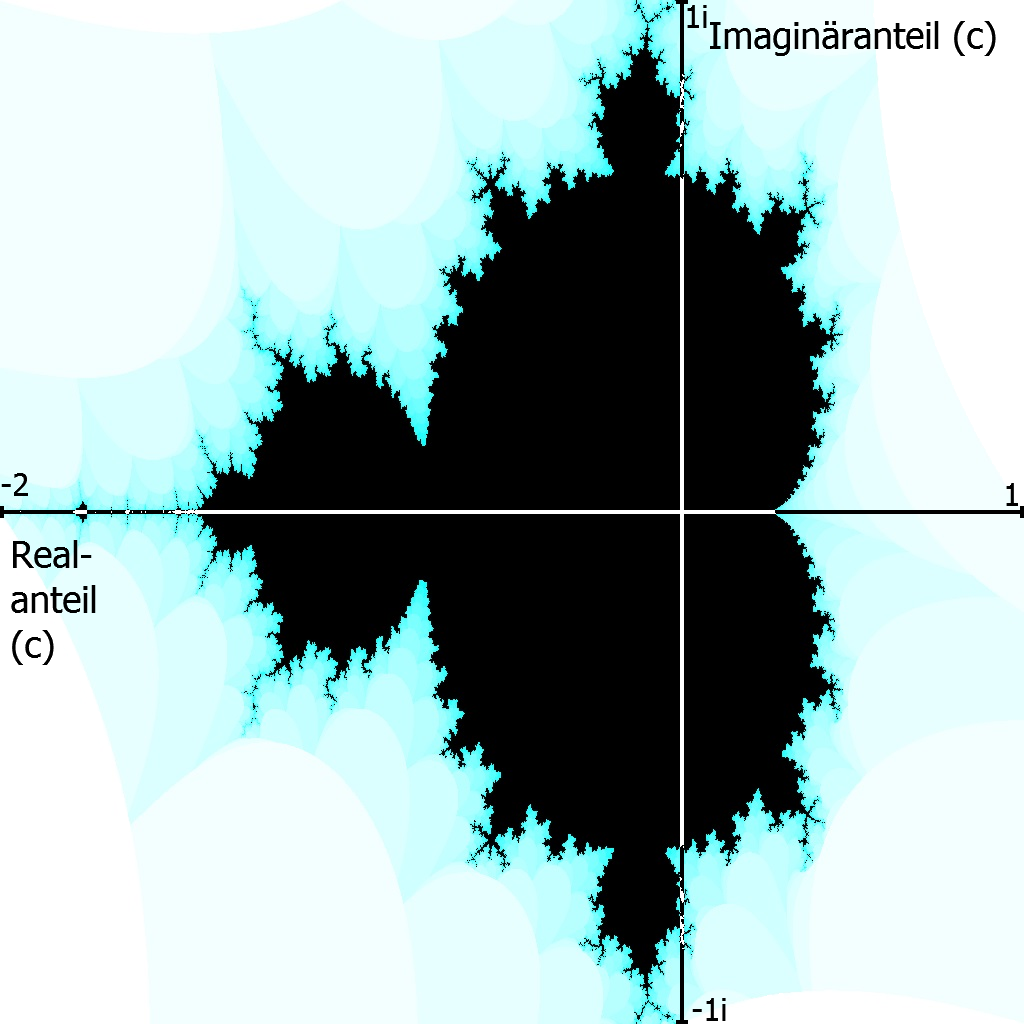
\includegraphics[scale=0.225]{pictures/MandelbrotMitAchsen.png}
\caption{Ausschnitt des Mandelbrotes in der komplexen Zahlenebene}
\label{fig:Mandelbrot}
\end{figure}

Um den Algorithmus umsetzen zu können, sollten wir uns vorher mithilfe dieser Informationen überlegen, wie Realteil und Imaginärteil von $z_{i+1}$ aus dem Real- sowie Imaginärteil von $z_i$ hervorgehen und diese Informationen danach als Iterationsvorschrift für unseren Algorithmus verwenden.
Je nachdem ob die Folge an einen Pixel beschränkt ist oder nicht, sollten wir den Pixel im Ausgabebild schwarz oder nicht schwarz färben.
Wie die Pixel, deren zugehörige komplexe Zahl nicht zur Mandelbrotmenge gehört, gefärbt werden blieb dabei uns überlassen. \\
Diese Aufgabenstellung spezifizierten wir noch an zwei Stellen.
Dazu zählt, dass wir als Auflösung für das auszugebende Bild nur Vielfache von Vier, welche größer als Vier sind, akzeptieren.
Außerdem haben wir noch festgelegt, dass all jene Pixel, deren zugeordnete komplexe Zahl nicht zur Mandelbrotmenge gehört, in einem blauen Farbton gefärbt werden, welcher von der Anzahl der auf ihnen durchgeführten Formeliterationen abhängt, die nötig waren, um festzustellen, dass sie nicht zur Mandelbrotmenge gehören.


\section{Lösungsfindung}
Nachdem bekannt gegeben wurde welche Aufgabe unser Team bekommt hat sich zunächst jeder für sich mit der Mandelbrotmenge an sich beschäftigt.
Das hat uns in sofern geholfen, dass als wir uns zur ersten Besprechung getroffen haben jeder schon eine Ahnung davon hatte was überhaupt zu tun ist.
Für uns alle war von vornherein die beste Möglichkeit an das Problem heranzugehen, zuerst das C-Programm mit Input und Output zu schreiben und uns dann an den Assembler-Teil setzen.

Dieser Assembler-Teil sollte zunächst nur eine sehr simple Version sein, um einen Überblick zu bekommen, welche Probleme wir bei der tatsächlichen Implementierung zu beachten haben.
Es stand somit fest, dass wir zwei verschiedene Versionen der Mandelbrotfunktion implementieren werden.
Auf diese Weise hatten wir von vornherein ein Programm was funktioniert ohne, dass wir Stubs oder Ähnliches benutzen müssen.
Wir hatten also ein Programm, was uns ein Bild mit bestimmten Maßen und korrekten Bildpunkten ausgibt.
Jedoch hatte das Bild noch nichts mit der Mandelbrotmenge zu tun, da wir diesen Teil nicht in dem C-Programm umgesetzt haben, was im Nachhinein in manchen Situationen recht hilfreich gewesen wäre.
Deshalb haben wir uns danach um den Assembler-Teil gekümmert.

Das Ziel war also das Array komplett unbeschrieben an die Assembler-Funktion zu übergeben und es dort dann korrekt zu befüllen und abzuspeichern.
Damit stellten wir sicher, dass wir später, wenn der Code komplexer wird, dieses Problem ausschließen können.
Da wir das Array zu diesem Zeitpunkt einfach nur von Bildpunkt zu Bildpunkt durchgelaufen sind, war es klar, dass wir nur noch den richtigen Farbwert an der Stelle ausrechnen müssten und es würde ein korrektes Bild ergeben.

Somit war der nächste Schritt sich konkret mit der Berechnung der Mandelbrotmenge zubeschäftigen und uns dazu eine Art Pseudo-Assembler-Code zuerstellen.
Dieser Pseudo-Code musste letztendlich nur noch angepasst und an der richtigen Stelle eingefügt werden.
Da wir nun einen funktionierenden Code hatten, der uns die Mandelbrotmenge richtig in einem Bild abspeichert, haben wir uns überlegt wie wir das Grundgerüst so umschreiben können, dass es parallel mehrere Pixel gleichzeitig berechnet.

Zunächst war die Idee ein float-Array zu initialisieren und dieses vorerst nur mit den Positionswerten für die einzelnen Berechnungen beschreibt.
Diese werden dann mit einem Structure-Load in die Q-Register geladen und dort parallel verarbeitet.

Da aber die korrekte Erstellung eines float-Arrays zu aufwändig ist und wir uns nicht sicher waren, ob wir es auch tatsächlich auf diese Weise zum Laufen bringen,
haben wir uns letzten Endes doch für die zweite Option entschieden.
Diese ist vermutlich die schnellste Art die Mandelbrotmenge parallel zu berechnen und war für uns alle gut zu verstehen.
Die Idee dahinter ist, dass man kontinuierlich 4 Pixel gleichzeitig berechnet und wenn einer von diesen rausfällt, weil er fertig berechnet ist, wird er sofort durch einen anderen Pixel ersetzt.
Somit muss das System nicht darauf warten, dass alle 4 Pixel fertig sind, aber die Implementierung wird im weiteren Verlauf noch genauer ausgearbeitet.
Mit dem gesammelten Wissen aus der simplen Single-Pixel Berechnung war die Implementierung dieser Version auch nicht mehr allzu kompliziert.
Nach ein paar Fehlerausbesserungen funktionierte nun also auch die zweite Version.


\section{Dokumentation der Implementierung}
\subsection{Implementierung des C-Programms}
Bevor wir zu der Umsetzung der Mandelbrotmenge kommen, wird zuerst die Ein/Ausgabe und Laufzeitanalyse in unserem C-Programm genauer erläutert.
Hierfür werden zuerst die einzelnen Methode genauer analysiert und anschließend wird der Ablauf in der Main-Methode spezifiziert.
Da wir zwei Assemblercodes für die Mandelbrotmenge implementiert haben, stehen die externen Verlinkungen zu diesen ganz oben.
In diesen werden die durch die Angabe spezifizierten Übergabeparamter von xStart, xEnd, yStart, yEnd und Auflösung bei beiden Aufrufen eingehalten.
Lediglich die Methodennamen weichen von der Vorgabe ab, aufgrund der unterschiedlichen Implementierungen.

Die Methode createBMP ist dafür verantwortlich unser zuvor berechnetes Array an Pixeln in eine Bitmapdatei zu speichern.
Hier ist zu beachten, wie das Dateiformat genauer spezifiziert ist \footnote{\label{not:wikiBMP}\url{https://en.wikipedia.org/wiki/BMP_file_format}, vom 27.01.2017}.
Zunächst wird ein Fileheader erstellt und initalisiert, anschließend erstellen wir den Infoheader.
Da in diesem die Dateigröße spezifiziert werden muss, berechnen wir die Größe des Bildes und addieren anschließend in einer seperaten Variable noch die Größe der beiden Header dazu.
Dies geschieht in zwei verschiedenen Variablen, da später die Größe des Bildes noch benötigt wird.
Da wir immer nur ein Byte auf einmal schreiben wollen, legen wir unsere Header so an, dass wir den Integerwert der Bildgröße in vier Byte speichern.
Das bedeutet, dass wir viermal die Größe schreiben müssen, jedoch immer geschiftet, damit die Bytes in der richtigen Reihenfolge im Header stehen.
Das gleiche geschieht bei Höhe, Breite und Bildgröße, welche im Infoheader geschrieben werden.
Anschließend benutzen wir die Standardmethoden von C um eine Datei zu öffnen, die beiden Header zu schreiben und anschließend das Bild anzuhängen.
Wichtig ist hier den Dateinamen mit .bmp zu beenden, damit das Bild später auch als Bild interpretiert werden kann.

In der nächsten Methode secondes erzeugen wir einen Zeitstempel.
Dieser wird als double für genauere Berechnungen zurück gegeben.
Um den Zeitstempel zu erzeugen verwenden bereits vorimplementierte C Methoden, mit welchen wir eine Genauigkeit im Bereich von Nanosekunden erhalten.

Um sicherzustellen, dass wir keine falschen Übergaben in unserem Programm verwenden, wurde eine Methode dafür entwickelt um Eingaben zu überprüfen.
Da ein Übergabeparameter zunächst ein String ist, versuchen wir bereits in diesem Fehler zu finden.
Hierfp wird die Länge des Strings bestimmt und anschließend jeder einzelne Character darauf überprüft ob er eine Zahl ist.
Da wir führende Nullen nicht zulassen, überprüfen wir den String auf solche.

Nach der Überprüfung auf die korrekte Anzahl an Übergabeparametern, werden zu Beginn in der Main-Methode fünf Variablen für die Übergabeparameter erstellt und mit Null initalisiert.
Anschließend erzeugen wir sechs Zeitstempel und setzen zunächst den ersten.
Vier der Zeiten dienen dazu die Gesamtlufzeit zu messen und die Laufzeit für das Berechnen der Menge selber.
Bevor wir die zuvor erstellten Variablen für die Übergabeparamter mittels einer C-Funktion in Integer umwandeln, werden diese mit der oben beschriebenen Funktion auf ihre Gültigkeit überprüft.
Sollte hierbei ein Fehler auftreten, so beendet sich das Programm und gibt eine Fehlermeldung aus.
Anschließend werden die Übergabeparameter noch auf ihre Gültigkeit gemäß unserer nachfolgenden Anforderung hin überprüft.
Hier gilt, dass ein Startwert immer kleiner sein muss als sein korrespondierender Endwert und die Auflösung nicht negativ oder foglende Definition nicht verletzen darf: $Aufl"osung$ $= 2^n$ $f"ur$ $n>2$.
Wurden alle Tests bis hierhin bestanden, wird der Benutzer dazu aufgefordert eine der beiden Berechnungsarten zu wählen.
Die verbrauchte Zeit bei der Eingabeaufforderung wird gemessen und am Ende von der Gesamtlaufzeit abgezogen, damit das Ergebnis nicht verfälscht wird.
Anschließend erstellen wir das Array und übergeben es an die gewünschte Umsetzung der Mandelbrotmenge.
Vor der Übergabe wird ein Zeitsstempel für den Beginn der Berechnung gesetzt un nach beenden dieser eine zweite Zeit gemessen.
Im Anschluss wird die Lauzeit des ausgewählten Algorithmus auf der Konsole ausgegeben.
Jetzt wird das berechnete Bildarray nur noch an die Spepicherfunktion übergeben, wo es wie oben erwähnt abgespeichert wird.
Bevor wir das Programm verlassen, wird die Gesamtlaufzeit noch berechnet und ebenfalls auf der Konsole ausgegeben.

\subsection{Implementierung Single-Pixel-Calculation}

\subsubsection{Konzept}

Die Idee hinter der Single-Pixel-Implementierung ist sehr unkompliziert und daher auch um einiges einfacher umzusetzen.
Es werden lediglich zwei Schleifen durchlaufen, welche jeweils die X-Achse bzw. die Y-Achse ablaufen. Wir berechnen also jeden Bildpunkt der zu berechnen und auszuwerten ist einzeln, daher auch der Name für die Funktion.
Das heißt, dass wir für den aktuell zu berechnenden Pixel sehr einfach an die Grundwerte für die Berechnung kommen, da wir bei jedem Schleifendurchlauf lediglich die X und Y Position durch eine Addition aktualisieren müssen.
Der X-Wert wird jedoch nach jedem vollständigen durchlaufen der X-Schleife auf seinen Grundwert zurückgesetzt.
Dieser Ablauf wird so lang ausgeführt bis die Y-Schleife einmal komplett durchlaufen wurde.

\subsubsection{Konkrete Umsetzung}
Zu Beginn werden die Register r4 bis r10, so wie das Link-Register auf dem Stack gesichert, damit, nachdem die Funktion wieder verlassen wurde, alles wieder dort ist wo es sein muss.
Bevor die eigentliche Arbeit anfangen kann benötigen wir lediglich die restlichen beiden Übergabewerte, welche nicht automatisch mit übergeben werden.
Diese bekommen wir mithilfe von zwei Loads und dem Stackpointer.
Nun haben wir alle benötigten Werte und beginnen damit die Schrittgröße in Y-Richtung zu berechnen.
Da die Schrittgröße jedoch meist nicht als eine Ganze Zahl dargestellt werden kann, sondern oft nur als Gleitkommazahl, müssen wir hierfür die s-Register benutzen.
Wir verschieben r3 nach s0 und berechnen mit einer simplen Subtraktion von r3 und r2 die Differenz zwischen iEnd und iStart, welche wir in r9 abspeichern.
Nun wird r9 nach s1 und r4 nach s4 verschoben. Die Werte dieser drei Register werden jetzt in ein 32-Bit float konvertiert.
So beinhaltet s0 jetzt iStart, s1 die Differenz, und s4 die im C-Teil spezifizierte Resolution.
Die Schrittgröße berechnet sich nun aus der Division der Differenz und der Resolution.
Jedoch ist für die richtige Berechnung eine kleine Anpassung an der Resolution vorzunehmen.
Wenn man von einer Resolution von 4 ausgeht sind es lediglich 3 Schritte die noch zu machen sind.
Das heißt wir müssen zunächst in r9 eine 1 abspeichern, r9 nach s5 kopieren, s5 in ein float konvertieren und s5 von s4 abziehen.
Nun muss lediglich die Division von s1 durch s4 durchgeführt werden und die Schrittgröße wird wiederum in s1 abgespeichert.
Für die Schrittgröße in X-Richtung wird das Selbe durchgeführt, mit dem einzigen Unterschied, dass die Resolution nicht mehr vorbereitet werden muss.

Die Vorbereitung ist getan, also kommt es jetzt direkt zu den Schleifen.
Wir beginnen damit einen Counter für die Y-Schleife mit dem Wert 0 zu initialisieren und setzen ein Label, um später wieder zu diesem Punkt zurückspringen zu können.
Das selbe machen wir für die X-Schleife, jedoch muss zuvor der Wert in s4, was in Zukunft die aktuelle X-Position speichert, auf den X-Startwert aus s2 zurückgesetzt werden.

Es folgt die eigentliche Berechnung des Bildpunktes, welche mit dem initialisieren der beiden Register s5 und s6 mit 0 beginnt, da man immer vom Punkt (0/0) startet.
s5 stellt den Imaginärteil dar und s6 den Realteil.
In r9 wird die maximale Anzahl an Durchläufen gespeichert und auf 20 gesetzt.
Ein letztes Label für die Berechnungs-Schleife. Nun wird s5 quadriert und in s7 abgespeichert, da wir diesen Wert einzeln benötigen.
Eine weitere Multiplikation von s5 und s6 welche anschließend verdoppelt wird und in s5 gespeichert wird.
Der Realteil wird auch quadriert, was durch eine Multiplikation von s6 mit sich selbst durchgeführt wird und in s8 abgespeichert wird.
Nun ziehen wir die beiden Quadrate von einander ab, also s8-s7 und speichern das Ergebnis in s6.
Für den nächsten Schleifendurchlauf müssen der Imaginär und Realteil noch mit den jeweiligen Konstanten, also den aktuellen Positionswerten addiert werden.
Anschließend wollen wir wissen, ob die Summe aus den beiden neuen Werten, welche sich in s5 und s6 befinden, eine bestimmte Grenze überschritten haben.
Dafür quadrieren wir die Summe um leichter Negative Zahlen behandeln zu können und vergleichen das Ergebnis mit 4.
Nun wird der Farbwert, welcher sich in r8 befindet, grundsätzlich auf 255 gesetzt, was einem weissen Pixel entspricht.
Daraufhin springen wir je nachdem, ob bei dem vorherigen Vergleich das Ergebnis größergleich 4 war, zum Schleifenabbruch, was ein Label am Ende der Berechnungsschleife ist.
Damit überspringen wir den Teil der also nur durchlaufen wird, wenn das Ergbnis kleiner 4 war. Dort wird nämlich der Farbwert auf 0, also Schwarz, gesetzt.
Zudem wird der Schleifencounter in r9 um 1 verringert und wir springen zurück an den Schleifen Anfang der Berechnung, falls der Counter noch nicht kleiner als 0 geworden ist.
Wenn der Counter jedoch kleiner 0 ist landen wir bei dem Label für den Schleifenabbruch, welcher zuvor erwähnt wurde.
Dort wird lediglich der Farbwert in das Array, auf das der Pointer in r5 zeigt, abgespeichert und der Pointer anschließend um 1 erhöht.

Somit ist die Berechnung für den Bildpunkt fertig und es kommt zum Schleifenende der X-Schleife.
Dort wird die X-Position um die zugehörige Schrittgröße erhöht, der Schleifencounter wird ebenfalls um 1 erhöht und anschließend mit der Resolution verglichen.
Falls der Wert noch kleiner ist als die Resolution branchen wir zurück zum X-Schleifenanfang.
Wenn nicht wird das selbe für die Y-Schleife ausgeführt.

Wenn wir hier wieder aus der Schleife rausfallen haben wir im Prinzip das Ende der Funktion erreicht.
Es muss lediglich der Stack wiederhergestellt und zum Link in das C-Programm zurückgebrancht werden.

\subsection{Implementierung Mult-Pixel-Calculation}


\subsubsection{Konzept}

Unser zweites Konzept basiert auf dem Prinzip eine dauerhafte Berechnung aufrecht zu erhalten.
Wie bereits zuvor erwähnt fällt ein Pixel unter zwei Bedingungen aus der Berechnung heraus. Erstens wenn von einem Pixel eine maximale Anzahl an Schleifendurchläufen mitgemacht wurden, oder zweitens wenn gilt:

\begin{equation*}
      (Imagin"arteil + Realteil)^2 > Schwellwert
\end{equation*}
Diese dauerhafte Berechnung wird nur dann unterbrochen wenn ein Pixel eines seiner Abbruchkriterien erfüllt.
Tritt dieser Fall ein besitzt jeder Pixel eine eigene Funktion. Diese speichert das Ergebnis des Pixels in das Bildarray und tauscht
mittels der festgelegten Register für Konstanten die notwendigen neuen Werte (Positionswerte, Speicheradresse) mit den alten aus. Außerdem wird auch noch sein Laufwert zurückgesetzt, da wir diesen benutzen um den Grad der Konvergenz zu ermitteln und die korrespondierenden Pixel blau zu färben.
Des Weiteren werden alle Werte für den neuen Pixel berechnet und gespeichert.
Hierbei war die Schwierigkeit einen Zeilenumbruch in den Pixelreihen zu erkennen und die daazugehörogen Laufwerte zu aktualisieren.
Mittels \autoref{fig:Konzept} soll das gerade beschriebene Konzept noch einmal vereinfacht dargestellt werden.
Im weiterem Verlauf wird nun auf die konkrete Implementierung unseres Konzeptes eingegangen.


\begin{figure}[ht]
  \begin{center}
    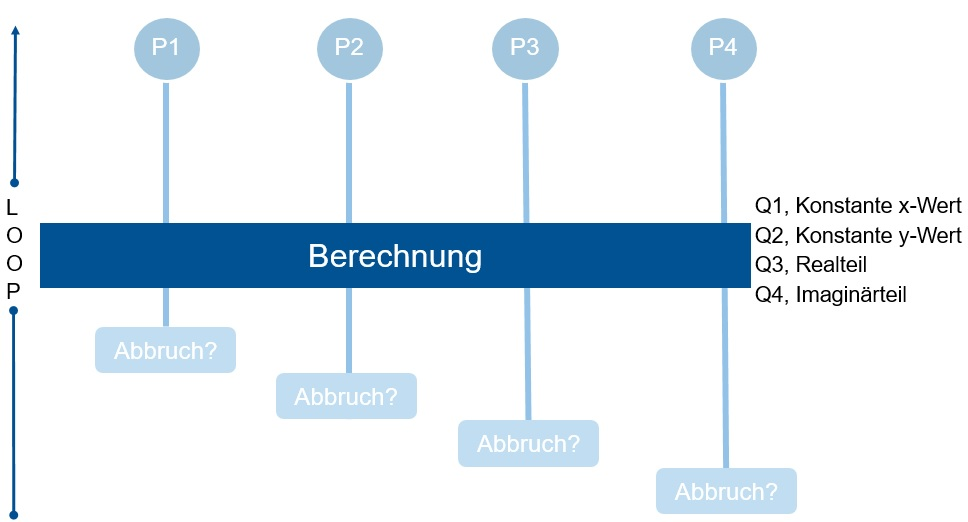
\includegraphics[width=12cm]{pictures/KonzeptLanes}
    \caption{Grafische Darstellung des Berechnungsprinzips:}
    \text{Durchlaufen der Berechnungsschleife von Pixel P1-P4,}
    \text{nach jeder Iteration werden die Pixel sequentiell auf Abbruch überprüft}
    \text{Bei einem Abbruch werden sie mit dem nächsten Pixel ausgetauscht}

    \label{fig:Konzept}
  \end{center}
\end{figure}

\subsubsection{Konkrete Umsetzung}
Bei unserer Umsetzung der Mandelbrotmenge  benutzen wir fast alle Resourcen, die uns der Prozessor zu verfügung stellt.
Konkret bedeutet das, dass wir alle zulässigen allgemeinen Register benötigen. Deshalb werden alle Register auf dem Stack gesichert. Das Link-Register wird auch abgesichert, damit ein Rücksprungsmöglichkeit in das C-Programm erhalten bleibt.
Da wir sechs Übergabewerte haben und nur die ersten vier automatisch in R0-R3 geladen werden, werden die letzten beiden Werte vom Stack ausgelesen.
Der Anfang der Multi-Pixel-Calculation ist größtenteils identisch mit dem der Single-Pixel-Camlculation.
Zu Beginn berechnen wir pro Achse die Strecke zwischen den Start- und Endwerten.
Mittels der Auflösung wird anschließend der Unterschied zwischen zwei Pixeln in der FPU berechnet.
Hierbei ist zu beachten, das wir von der Auflösung zuvor eine Kopie erstellt welche um den Wert eins verringert wurde, da ansonsten immer das letzte Pixel einer Reihe nicht auf dem Endpunkt liegt sondern einen Abstand davor.
Das Register q0 wurde anschließend als Register für Variablen festgelegt, welche während der dauerhaften Berechnung benötigt werden.
Die freien allgemein Register werden nun für die Hauptberechnung initalisiert.
Da zu Beginn fesgelegt wurde, dass die Größe des Bildes immer $Aufl"osung^2$ ist, wird in Register zwei diese gespepichert.
Register zwei ist also der Schleifenlaufwert, welcher verwendet wird um festzustellen, wann alle Pixel berechnet sind.
Die weiteren Register drei bis sechs enthalten die Anzahl der bereits durchlaufenen Iterationen.
Die Maximale Anzahl an erlaubten Iterationen wird in dem darauffolgendem Register R7 gespeichert.
Somit ist es später möglich mit diesen Registern das bereits oben erwähnte Abbruchkriterium der maximalen Iterationsdurchläufe zu realisieren.
Die Register R8-R11 werden nun mit der für den Pixel entsprechenden Speicheradresse initalisiert.
Hierbei ist zu beachten, dass R0 immer den Wert enthält für den nächsten Pixel nicht für den letzten.
Es werden vier seperate Speicheradressen deshalb verwendet, da während der Berechnung die Pixel nicht immer gleich lang brauchen und somit Pixel4 vor Pixel1 fertig sein kann.
Würde man eine einzelne Speicheradresse dafür verwenden, würde die Reihenfolge das berechnenten Pixel im Bildarray nicht mehr stimmen.
Um das Problem zu lösen müsste Pixel4 bei schnellerer Berechnungszeit auf die Berechnung von Pixel1 warten, was viel Zeit kosten kann.
Um die Vorbereitungen für die Hauptberechnung abzuschließen werden die beiden float-Register s30 und s31 initalisiert.
In s30 steht der aktuelle x-Wert, also der Wert der zuletzt verwendet wurde und in s31 wurde der Schwellwert geschrieben.
Die \autoref{tbl: Allg} und \autoref{tbl: FPU} zeigen eine Übersicht über die allgemein und floating-point Register während der Berechnung.


Damit die Hauptschleife zu Beginn keinen Leerdurchlauf durchführt, werden vor Beginn der Schleife die entsprechenden Register (siehe: \autoref{fig:Konzept}) mit den ersten vier Pixelkoordinaten befüllt.
Damit es zu keinen Fehlern in der maximalen Anzahl an zu berechnenden Pixeln kommt, werden bereits nach der Berechnung von R2 diese vier Pixel abgezogen.
Demnach stehen jetzt in q1 und q2 die x-Werte bzw. y-Werte. Somit bilden q1, q2 unser Konstante. Da die erste Iteration der Schleife als Ergebniss die Konstante selber ist kann man diese Überspringen, indem man in die Register q3 (Realteil von $z_i$) und q4 (Imaginärteil von $z_i$) direkt in die Konstante kopiert.
Das Überspringen der ersten Iteration wird auch bei einem Pxielwechsel umgesetzt. Dadurch lässt sich pro Pixel eine Iteration einsparen, was sich später positiv auf die Laufzeit auswirkt.


Zu diesem Zeitpunkt wird nun die Schleife gestartet.
Um die binomische Formel von $(z_i)^2 = (a*i+b)^2= b^2 - a^2 + 2*a*b$ zu realisieren wird q5 als Zwischenspeicher von $2*a*b$ verwendet.
Wir berechnen $2*a*b$ zuerst, da wir dadurch nur ein Register als Zwischenspeicher benötigen.
Somit können die Register die Real- und Imaginärteil beinhalten anschließend quadriert Werden. Gemäß der Formel werden nun die neuen Real- und Imagonärteile berechnet.
Damit ist die eigentliche Berechnung von einer Iteration zu Ende.


Der weitere Teil an parallelen Schritten innerhalb von NEON dient dazu das zweite Abbruchkriterium zu testen.
In q5 werden nun Real und Imaginärteil aufsummiert und anschließend das Quadrat der Summe in q6 berechnet.
Hier wird das Quadrat verwendet, da somit nicht auf Divergenz von negative Zahlen getestet werden muss. Der Schwellwert wurde zuvor so ausgewählt, das dieser bereits das Quadratische des eigentlichen Schwellwertes ist.
Im weiteren Verlauf erfolgen nun die sequentiellen Überprüfungen des Pixels gemäß der Abbruchbedingungen.
Da die Überprüfung des einzelnen Pixel vom Aufbau her gleich ist, wird hier nur auf die Überprüfung eines Pixels eingegangen.
Die sequentielle Überprüfung aller vier Pixel ist allerdings notwendig, da in den gespeicherten Variablen in r0, q0 und q7 immer nur die Koordinaten für das nächste Pixel stehen.
Als erstes erfolgt die Überprüfung auf den Schwellwert, da dieser Fall häufiger eintritt und sich somit erneut ein paar Rechenoperationen einsparen lassen.
Ist diese Überprüfung erfolgreich, springen wir in die Funktion earlybailout des jeweiligen Pixels.
In dieser wird aufgrund der in R8-R11 gespepicherten Adressen die ersten beiden Bytes des Pixels mit dem $maximalenFarbwert=255$, für weiß initalisiert.
Um nun den Grad der Divergenz zu erhalten wenden wir folgende Formel an:

\begin{equation*}
    zu speichernder Farbwert = maxFarbwert -( 12*Anzahl der Schleifendurchl"aufe )
\end{equation*}
Die Zwölf ergibt sich aus der Ganzzahldivision des maximalen Farbwerts durch die maximale Anzahl an Schleifendurchläufen.
Das Ergebis wird anschließend an die Stelle des dritten Byte gespeichert.
Sollte jedoch die andere Abbruchbedingung eintreten, auf welche im Anschluss geprüft wird. so werden and die gespeicherte Speicheradresse der minimale Farbwert null gespeichert, was in einen schwarzen Pixel resultiert.
Dies geschieht in der maxBailout Funktion des jeweiligen Pixels.

Wenn ein Pixel nun fertig berechnet und seine Werte in das Bildarray gespeichert wurden, muss er mit dem nächsten zu berechnenden Pixel ausgetauscht werden.
Das Austauschen erfolgt in der jeweiligen Reset Funktion.
In dieser wird zunächst der Laufwert auf -1 gesetzt.
Der Laufwert wird nicht auf null gesetzt, da wir in der Hauptschleife erst nach allen Überprüfungen die Laufwerte inkrementieren und somit bei der ersten Iteration des neuen Pixels mit dem Laufwert 0 beginnt.
Der nächste Schritt ist die Überprüfung auf einen Zeilenumsprung.
Da uns die Länge einer Zeile bekannt ist, passiert dann ein Zeilenumbruch wenn gilt:

\begin{equation*}
  restlicheAnzahl an Pixeln \% Aufl"osung = 0
\end{equation*}

Da die vorhandene ARM-Architektur keine passende Modulo Operation bietet und auch keine Division von Ganzahlen unterstützt wird die standardmässig vorimplementierte Funktion des gcc-Compilers für zwei unsigned Integer Werte verwendet.
Mittels der Multiply wand Subtract Instruktion (MLS) kann man jetzt den Rest einer Division berechnen.
Ist das oben genannte Kriterium erfüllt, so findet ein Zeilenumbruch statt.
Bei diesem werden der aktuelle y-Wert um einen Schritt erhöht und der aktuelle x-Wert auf $StartX - xSchritt$ gestzt.
Das Setzen des x-Wertes ergibt sich daraus, das wir im weitern Vorgehen des Initalisierens des neuen Pixels, den x-Wert standardmäßig um einen Schritt erhöhen.
So ist gewährleistet, dass der neue Pixel bei xStart beginnt.
Am Schluss wird nun die neue Konstante gespeichert und aus den bereits vorher erwähnten Gründen die Konstante auch in Real- und Imaginärteil kopiert.
Auch der neue zu speichernde Adressbereich wird aktualisiert.

Sobald eines der beiden Abbruchkriterien eintritt wird auf das nächste Kriterium hin nicht mehr überprüft.
Sonst kann der noch nicht berechnete neue Pixel direkt gespeichert werden.
Nachdem alle Pixel überprüft wurden, erhöhen wir deren Laufwerte um eins und verifizieren ob wir noch weitere Berechnungen durchführen müssen.
Der gerade geschilderte Ablauf passiert solange bis wir alle Pixel berechnet haben.
Wurden alle benötigten Berechnungen durchgeführt so stellen wir den Ausgangszustand wieder her und springen zurück in das C-Programm.

\subsection{Anwendung des Programmes}

Um jetzt die bereits detailliert beschriebene Implementierung der Mandelbrotmenge zu verwenden, muss man das Programm mittels des Makefile compilieren. Der Programmaufruf erfolgt dann mittels der Konsole mit folgenden Übergabeparametern:
\begin{center}
  xStart: Integerwert der den Anfangswert auf der x-Achse repräsentiert

  xEnd: Integerwert der den Endewert auf der x-Achse repräsentiert

  yStart: Integerwert der den Anfangswert auf der y-Achse repräsentiert

  yEnd: Integerwert der den Endewert auf der y-Achse repräsentiert

  Auflösung: Integerwert für den gelten muss $Aufl"osung$ $= 2^n$ $f"ur$ $n>2$
\end{center}

Ein konkreter Aufruf wäre {\textbf./main -2 1 -1 1 1024}.
Für die jeweiligen Start- bzw Endwerte muss gelten, dass $Start < End$.
Wird bei der Auflösung für n ein Wert größer als 12 gewählt, so wird das Bild berechnet jedoch steigt die Zeit, die dafür benötigt wird, sehr schnell an.
Während man das Programm laufen lässt wird man aufgefordert sich ziwschen der Single-Pixel-Calculation oder der parallelisiserte Version zu entscheiden.
Am Ende erhält man ein Datei des .bmp Formates. Diese kann man sich jetzt mit dem bevorzugten Programm für Bilder anschauen.
Sollten für das Programm fehlerhafte Aufrufe durchgeführt werden oder während der Ausführung so beendet sich das Programm und muss neu aufgerufen werden.

\begin{table}
  \begin{center}
    \begin{tabular}{| l | l |}
      \hline
      R0 & Speicheradresse zum nächsten Pixel \\ \hline
      R1 & Auflösung\\ \hline
      R2 & Anzahl der Restlichen zu berechnenden Pixel \\ \hline
      R3 & Durchlaufene Iterationen Pixel 1 \\ \hline
      R4 & Durchlaufene Iterationen Pixel 2 \\ \hline
      R5 & Durchlaufene Iterationen Pixel 3 \\ \hline
      R6 & Durchlaufene Iterationen Pixel 4 \\ \hline
      R7 & Maximale Anzahl an erlaubten Iterationen \\ \hline
      R8 & Speicheradresse von Pixel 1 \\ \hline
      R9 & Speicheradresse von Pixel 2 \\ \hline
      R10 & Speicheradresse von Pixel 3 \\ \hline
      R11 & Speicheradresse von Pixel 4 \\ \hline
      R12 & allzweck Register zum berechnen oder zur Farbwertspeicherung \\ \hline
    \end{tabular}
  \end{center}

  \caption{Einteilung der allzweck Register zur Berechnungszeit}
  \label{tbl: Allg}
\end{table}

\begin{table}[!ht]
  \begin{center}
    \begin{tabular}{| l | l | l |}
      \hline
      q0 & s0 & Der Startwert auf der x-Achse \\ \cline{2-3}
      & s1 & Abstand zwischen zwei Pixeln entlang der x-Achse \\ \cline{2-3}
      & s2 & Aktuelle y-Position\\ \cline{2-3}
      & s3 & Abstand zwischen zwei Pixeln entlang der y-Achse\\ \hline

      q1 & s4 & Pixel 1 x-Position / Konstante Realteil \\ \cline{2-3}
      & s5&  Pixel 2 x-Position / Konstante Realteil\\ \cline{2-3}
      & s6&  Pixel 3 x-Position / Konstante Realteil\\ \cline{2-3}
      & s7&  Pixel 4 x-Position / Konstante Realteil\\ \hline

      q2& s8&  Pixel 1 y-Position / Konstante Realteil\\ \cline{2-3}
      & s9&  Pixel 2 y-Position / Konstante Realteil\\ \cline{2-3}
      & s10&  Pixel 3 y-Position / Konstante Realteil\\ \cline{2-3}
      & s11&  Pixel 4 y-Position / Konstante Realteil\\ \hline

      q3& s12&  Pixel 1 $z_i$ Realteil\\ \cline{2-3}
      & s13& Pixel 2 $z_i$ Realteil\\ \cline{2-3}
      & s14& Pixel 3 $z_i$ Realteil\\ \cline{2-3}
      & s15& Pixel 4 $z_i$ Realteil\\ \hline

      q4& s16& Pixel 1 $z_i$ Imaginarteil\\ \cline{2-3}
      & s17&  Pixel 2 $z_i$ Imaginarteil\\ \cline{2-3}
      & s18&  Pixel 3 $z_i$ Imaginarteil\\ \cline{2-3}
      & s19&  Pixel 4 $z_i$ Imaginarteil\\ \hline

      q5& s20& Berechnung Pixel 1: $2*a*b$ / Realteil+Imaginärteil \\ \cline{2-3}
      & s21& Berechnung Pixel 2: $2*a*b$ / Realteil+Imaginärteil\\ \cline{2-3}
      & s22& Berechnung Pixel 3: $2*a*b$ / Realteil+Imaginärteil\\ \cline{2-3}
      & s23& Berechnung Pixel 4: $2*a*b$ / Realteil+Imaginärteil\\ \hline

      q6& s24& Pixel 1: $(Imagin"arteil + Realteil)^2$ / Abbruchtest gegen Schwellwert\\ \cline{2-3}
      & s25& Pixel 2: $(Imagin"arteil + Realteil)^2$ / Abbruchtest gegen Schwellwert\\ \cline{2-3}
      & s26& Pixel 3: $(Imagin"arteil + Realteil)^2$ / Abbruchtest gegen Schwellwert\\ \cline{2-3}
      & s27& Pixel 4: $(Imagin"arteil + Realteil)^2$ / Abbruchtest gegen Schwellwert\\ \hline

      q7& s28& unbenutzt\\ \cline{2-3}
      & s29& unbenutzt\\ \cline{2-3}
      & s30& Aktuelle x-Position\\ \cline{2-3}
      & s31& Schwellwert\\ \hline

    \end{tabular}
  \end{center}
  \caption{Einteilung der NEON/FPU-Register zur Berechnungszeit}
  \label{tbl: FPU}
\end{table}


\clearpage
\section{Ergebnisse / Fazit}
\subsection{Ergebnisse und Optimierung}

Nachdem wir unsere parallele Implementierung fertiggestellt hatten, beginnen wir damit unsere beiden Programme zu vergleichen.
Mit der implementierten Laufzeitanalyse wurden für alle zulässigen Auflösungen zwischen 8 und 8192 die Laufzeit von beiden Berechnungsarten zehn mal gemessen.
Anschließend wurde der Mittelwert aus den zehn erhaltenen Zeiten gebildet und miteinander verglichen.
In \autoref{fig:v-Vergleich} wurde die Laufzeit der Single-Pixel-Calculation durch die der parallelen Berechnung geteilt um somit einen Faktor zu erhalten um wie viel schneller die Multi-Pixel-Calculation ist.
Zunächst nahmen wir an, dass die einfache Berechnung in den niedrigen Auflösungsbereichen schneller als die parallele sei. Jedoch zeigt sich auch in diesen Bereich, dass die parallele Berechnung schneller ist.
Allerdings erwartet man, dass sie circa drei mal so schnell sei, da anstelle von einem Pixel vier Pixel auf einmal bearbeitet werden.
Diese Diskrepanz lässt sich dadurch erklären, dass die NEON-Einheit für die parallele Berechnung zusätzliche Schritte unternehmen muss um die Berechnungen parallel durchzuführen.
Die durschnittliche halbierung der Laufzeit ist in etwa das, was am Ende zu erwarten war.

\begin{figure}[!ht]
  \begin{center}
    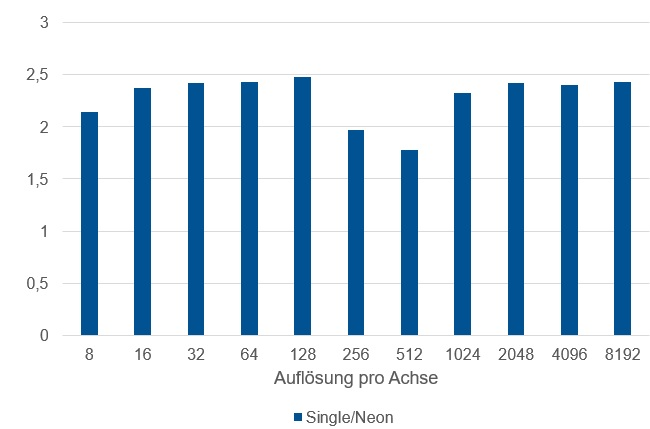
\includegraphics[width=10cm]{pictures/Geschwindigkeitsvergleich}
  \end{center}
  \caption{Vergleich von paralleler Berechnung zur einfachen Berechnung}
  \label{fig:v-Vergleich}
\end{figure}


Da wir bei unserer Implementierung eher den Ansatz verfolgt haben die Laufzeit zu minimieren sind wir nicht Speichereffizient, was die Anzahl an Register angeht.
So finden sich in dieser Hinsicht einige Möglichkeiten der Optimierung.
Als erster Ansatzpunkt wäre das Vereinigen der Pixelabbruchfunktionen.
Hier ist es sicherlich möglich auf Kosten von Laufzeit eine einheitliche Funktion zu schreiben.
Außerdem könnte man auch Speicheradressen auf den Stack auslagern und diese nur bei Bedarf laden und wieder absichern.
In Bezug auf Speichereffizienz im Hauptspeicher, benutzen wir das Minimum was unserer Meinung nach möglich ist, in Bezug auf die Speicherung einer bitmap Datei im Arbeitsspeicher.
An dieser Stelle haben wir die Aufgabenstellung so interpretiert, dass das die Ausgabefunktion nur das tatsächliche Array ohne weiter Berechnungen schreibt.
Ist dies nicht der Fall lässt sich der Speicher auf $1/3$ des ursprünglich benötigten Speichers verkleinern.
Da nun nur noch gespeichert werden muss ob das Pixel konvergiert oder nicht.
Beim Abspeichern des Bildes in C müsste man dann nur noch die Pixelfarben entsprechend dem Eintrag berechnen und die drei Bytes in die Bitmapdatei schreiben.

\section{Zusammenfassung des Projektes}
Im Laufe des Projektes haben wir Schritt für Schritt einen funktionierenden Algorithmus entworfen und implementiert, der zur Berechnung der Mandelbrotmenge  genutzt werden kann.
Ausgehend von einer prototypischen Implementierung in Pseudocode entwickelten wir zunächst einen funktionierenden Algorithmus in Assembler, welcher noch eine schlechte Performanz aufwies.
Diesen Algorithmus optimierten wir im darauffolgenden Schritt unter den Gesichtspunkten Laufzeit und Speichernutzung.
Nach dem Vorbild dieser optimierten Version begannen wir im nächsten Schritt eine parallelisierte Berechnung durch Verwendung von NEON/SIMD-Befehlen zu entwerfen.
Dabei entstanden zwei verschiedene Ansätze, die sich in den Punkten „Einfachheit der Umsetzung“ und „Laufzeit“ deutlich unterschieden.
Letztendlich entschieden wir uns gegen den Ansatz, in dem eine blockweise Parallelberechnung der Pixel vorgesehen war, und für den Ansatz, in welchem die Berechnung für mehrere Pixel gleichzeitig aber nicht blockweise abläuft.
Dadurch werden bereits fertig berechnete Pixel durch den nächsten unberechneten Pixel ersetzt.
Diese Variante haben wir effektiv umgesetzt.
Zum Schluss haben wir unsere Implementierung noch so abgeändert, dass nicht nur ausgegeben wird, ob an einem Pixel die dazugehörige komplexe Zahl zur Mandelbrotmenge gehört, sondern auch ab welcher Anzahl an Iterationen erkannt wurde, dass sie nicht dazu gehört.


Im Groben und Ganzen würden wir sagen, dass unser Programm zeiteffizient ist und eine saubere, funktionierende Implementierung der Berechnung der Mandelbrotmenge umsetzt.
Diese weist allerdings noch einige Möglichkeiten zur Verbesserung auf.
Wie im bisherigen Text bereits erwähnt könnte man die Speichernutzung des Algorithmus verbessern, indem man einige selten genutzte Werte nicht in den Registern sondern auf den Stack auslagert und sie gegebenenfalls wieder lädt.
Außerdem berücksichtigt unser Programm nicht die Seitenverhältnisse des Mandelbrotausschnitts bei der Berechnung. Das bedeutet, dass auch bei der Berechnung auf nicht quadratischen Abschnitten der komplexen Zahlenebene ein quadratisches Bild ausgegeben wird.
Ebenfalls könnte man den Algorithmus noch insofern verbessern, dass er auch andere Auflösungen als nur Vielfache von Vier, die größer als Vier sind, erlaubt und zu diesen ein korrektes Bild erstellt.
Zudem ist der Assemblercode noch teilweise redundant und könnte übersichtlicher gestaltet werden.
\pagebreak




\end{document}
